% mpc_cuda_report.en.tex -- technical report (English)
% Build: uplatex mpc_cuda_report.en.tex && dvipdfmx mpc_cuda_report.en
\documentclass[uplatex,dvipdfmx,a4paper,11pt]{jsarticle}
\usepackage{amsmath,amssymb}
\usepackage{booktabs}
\usepackage{array}
\usepackage{listings}
\usepackage{url}
\usepackage[dvipdfmx]{graphicx}
\usepackage[dvipdfmx]{xcolor}
\usepackage[dvipdfmx,colorlinks=true,linkcolor=blue,citecolor=blue,urlcolor=blue]{hyperref}

\lstset{
  basicstyle=\ttfamily\small,
  frame=single,
  breaklines=true,
  columns=fullflexible,
  keepspaces=true,
  showstringspaces=false,
  xleftmargin=1.5em,
  framexleftmargin=1.5em,
}
\newcommand{\code}[1]{\texttt{#1}}

\title{mpc\_cuda: Porting GMP/MPFR/MPC to CUDA\\
{\large ---- Construction, Implementation Difficulties, and Performance ----}}
\author{tkouya}
\date{\today}

\begin{document}
\maketitle

\begin{abstract}
This report describes \textbf{mpc\_cuda}, a port of the GNU multiple-precision
stack---GMP, MPFR and MPC---that runs inside NVIDIA CUDA kernels. We cover the
construction procedure, the implementation difficulties met during the port and
their solutions, and a performance evaluation of basic linear algebra and
elementary functions. We further introduce a compile-time fixed-precision,
register-resident fast path, \code{cu\_freal<PB>}/\code{cu\_fcomplex<PB>}, and
quantify the GPU/CPU performance crossover over the precision range
128--8192 bits. The primary hardware is the NVIDIA GB10 (compute capability 12.1,
\code{sm\_121}, CUDA 13); we additionally cross-compare the runtime-precision
demos against an NVIDIA H100 NVL (compute capability 9.0, \code{sm\_90}). All
results are bit-identical to host MPFR/MPC (or within $\le 1$ ULP for the
elementary functions).
\end{abstract}

\tableofcontents
\bigskip

%======================================================================
\section{Introduction}
\label{sec:intro}

Running arbitrary-precision arithmetic on the GPU is attractive for the
numerical linear algebra of ill-conditioned problems and for high-precision
simulation. Existing GPU multiple-precision libraries (e.g.\ CUMP ports GMP's
\code{mpf}) exist but often have loose rounding semantics and lack complex
numbers and elementary functions. The goal of this project is to run the
\textbf{correctly-rounded real semantics of MPFR}, and \textbf{the complex MPC
layer on top of it}, inside CUDA kernels as \textbf{faithfully} as possible
(a port of the upstream sources, not a reimplementation). Concretely, the target
was to evaluate \code{y = a\,x + y} (AXPY) for both real (MPFR) and complex (MPC)
operands on the GPU, match the CPU result bit-for-bit, and obtain a substantial
speedup.

The report is organised as follows. Section~\ref{sec:procedure} describes the
overall design and construction procedure (the transform-script approach and the
layered phases). Section~\ref{sec:difficulties} details the porting difficulties
and their solutions. Section~\ref{sec:fixed} presents the compile-time
fixed-precision fast path, and Section~\ref{sec:perf} the performance evaluation
(AXPY, linear algebra, elementary functions, and the precision sweep).
Section~\ref{sec:conclusion} concludes.

%======================================================================
\section{Overall Design and Construction Procedure}
\label{sec:procedure}

\subsection{The upstream sources}

The base of the port is \textbf{mini-gmp} (\code{gmp-6.3.0/mini-gmp}), a subset
implementation of GMP. mini-gmp provides, in a single C source, the core of
\code{mpz} (multiple-precision integers) and \code{mpn} (low-level limb arrays).
MPFR-4.2.2 builds on mini-gmp with \code{--with-mini-gmp}; the few missing
\code{mpn} routines (\code{mpn\_divrem}, etc.) are supplied by MPFR's own
\code{mpfr-mini-gmp.c}. Thus \textbf{no full-GMP internals are required}.
MPC-1.4.1 is the thin complex layer on top of MPFR and rides the same base.

\subsection{The transform-script approach}

Hand-forking the upstream sources makes it hard to re-apply upstream updates.
Instead this project performs device adaptation through \textbf{re-runnable
transform scripts} (\code{tools/cudafy\_*.py}).

\begin{itemize}
\item \code{tools/cudafy\_minigmp.py}: reads the pristine \code{mini-gmp.\{c,h\}}
      and emits \code{include/mpc\_cuda/cuda\_minigmp.h} and
      \code{src/cuda\_minigmp.cu} with \code{\_\_host\_\_ \_\_device\_\_} prepended
      to every device-reachable function. Host-only functions (those using
      stdio/realloc/ctype) are detected by a word-boundary token scan.
\item \code{tools/cudafy\_mpfr.py}: applies the same adaptation to MPFR's 263
      sources.
\item \code{tools/cudafy\_mpc.py}: applies it to MPC's 90 sources (reusing the
      MPFR machinery).
\end{itemize}

This keeps the upstream structure intact, so re-running the scripts re-applies
upstream updates.

\subsection{The layered phases}

Development proceeded in four phases (plus 2b), each validated bit-for-bit
against the host before building on it.

\begin{table}[h]
\centering
\caption{The layered development phases}
\begin{tabular}{clp{7.5cm}}
\toprule
Phase & Layer & Content \\
\midrule
1  & mini-gmp & \code{mpz}/\code{mpn} on the device. add/sub/mul/tdiv\_qr/pow\_ui/get\_str bit-exact vs host (256 threads).\\
2  & MPFR (faithful) & Real \code{mpfr-4.2.2} init2/set/mul/add/get\_d run inside kernels.\\
2b & MPFR transcendentals & pi/exp/log/sin/cos/atan/sqrt work (requires the \code{mpfr\_div} substitution below).\\
3  & MPC (complex) & Real \code{mpc-1.4.1} init2/set\_d\_d/mul/add run.\\
4  & AXPY demos / benchmarks & Real and complex AXPY, GPU vs CPU, time and accuracy.\\
\bottomrule
\end{tabular}
\end{table}

%======================================================================
\section{Implementation Difficulties and Solutions}
\label{sec:difficulties}

``It compiles'' and ``it runs correctly on the device'' are different problems.
This section classifies the difficulties that were the crux of the port.

\subsection{Making it compile}

\begin{enumerate}
\item \textbf{C11 \code{\_Noreturn}}: rejected by nvcc's C++ frontend. The
      host build's \code{-DMPFR\_HAVE\_NORETURN} must be \textbf{dropped}.
\item \textbf{Inline assembly}: the x86\_64 \code{umul\_ppmm} etc.\ in
      \code{mpfr-longlong.h} are invalid on the device. \code{-DNO\_ASM} selects
      the portable C fallbacks.
\item \textbf{No \code{realloc}}: CUDA device code has no \code{realloc}; it is
      emulated by malloc+memcpy+free (\code{mg\_cuda\_realloc}).
\item \textbf{C99 \code{\_Complex}}: device code has no \code{\_Complex}. MPC's
      \code{mpc.h} \code{\#if 1} (which defines \code{\_MPC\_HAVE\_COMPLEX\_H}) is
      turned into \code{\#if 0}, disabling \code{mpc\_set\_dc}/\code{get\_dc}.
\item \textbf{\code{gmp.h} shim}: MPC's \code{mpc.h} \code{\#include}s
      \code{gmp.h}. A shim pointing at the CUDA mini-gmp is generated, declaring
      minimal \code{gmp\_randstate\_t}/\code{mpf\_t}/\code{mpq\_t} stand-ins (absent
      from mini-gmp) so the prototypes parse.
\item \textbf{Token pasting}: MPC's \code{set\_x.c}/\code{set\_x\_x.c} expand
      \code{mpfr\_set\_\#\#type} for all setters in one TU, pulling in
      \code{mpfr\_set\_f}/\code{\_q} (absent under mini-gmp). Trapping device stubs
      are injected so the unit compiles.
\end{enumerate}

\subsection{Making it run correctly on the device}

This is the substantively hard part: even when it compiles, host-oriented global
state, function pointers, and optimisations misbehave on the device.

\begin{enumerate}
\item \textbf{Lookup tables}: file-scope \code{static const} arrays such as
      \code{invert\_limb\_table} and \code{\_\_clz\_tab} cannot be referenced from
      the device. They are tagged \code{MPFR\_RODATA} (\code{\_\_device\_\_} in the
      device pass, empty in the host pass), so one definition serves both passes.
\item \textbf{Global state}: \code{\_\_gmpfr\_emin}/\code{emax}/\code{flags} and the
      default precision/rounding become \code{\_\_device\_\_ \_\_managed\_\_}
      (shared host/device).
\item \textbf{assert/abort}: \code{mpfr\_assert\_fail} (fprintf+abort) and
      \code{gmp\_die} become \code{\_\_trap()} on the device.
\item \textbf{\code{\_\_builtin\_unreachable} miscompile}: enabling
      \code{MPFR\_HAVE\_BUILTIN\_UNREACHABLE} makes its
      \code{\_\_builtin\_constant\_p}/\code{\_\_builtin\_unreachable} path
      \textbf{miscompile} \code{MPFR\_ASSERTN} on the device (a provably-true
      assertion fired). Dropping the define fixes it.
\item \textbf{Allocation routing} (the subtle one): in mini-gmp mode
      \code{mpfr\_allocate\_func} (\code{mpfr-gmp.c}) fetches mini-gmp's allocation
      hooks via \code{mp\_get\_memory\_functions()}---\textbf{host function
      pointers}. Calling them from the device returned garbage (e.g.\ echoing the
      size, \code{0x28}). Patched so that under \code{\_\_CUDA\_ARCH\_\_} the
      allocate/reallocate/free funcs call the device heap directly.
\item \textbf{Constant caches}: \code{mpfr\_const\_pi/log2/euler/catalan} hold a
      compute-function \textbf{pointer} (a host address) at static init and memoise
      into a shared mutable global---an illegal instruction / data race on the
      device. They are rerouted to cacheless wrappers
      \code{mpfr\_const\_*\_cuda} that do \code{MPFR\_SAVE\_EXPO} (required---else
      the constants come out wrong) and call \code{*\_internal} directly.
\end{enumerate}

\subsection{The hardest problem: device miscompile of \code{mpfr\_div}}

The deepest problem was that \textbf{\code{mpfr\_div}'s generic path
(precision $\ge 3$ limbs) miscompiles on the device and returns \code{inf}/garbage}
while \textbf{the same code is correct on the host}. It cascaded:
\code{const\_pi}/\code{const\_log2} divide internally, so they came out
wrong/crashed (the earlier \code{const\_pi}-derived \code{mpn\_sqrtrem p[n-1]==0}
assertion was a \textbf{downstream symptom}---the broken quotient fed an
unnormalised value into the AGM's \code{mpfr\_sqrt}), which blocked
\code{log, sin, cos, atan, large exp}.

Exhaustive bisection confirmed every sub-primitive was \textbf{correct standalone
on the device} (\code{mpn\_divrem\_1}, \code{mpn\_divrem}, mini-gmp \code{mpz}
division, \code{count\_leading\_zeros}, \code{udiv\_qrnnd}, \code{MPFR\_TMP});
\code{-O0}/\code{-G} did not help; and the miscompiled construct resisted
statement-level isolation (instrumented writes were reordered/dropped around the
calls). Rather than chase the nvcc codegen issue, we \textbf{substituted a
self-contained, correctly-rounded \code{mpfr\_div} built only on \code{mpz}
primitives} (\code{mpfr\_div\_cuda}). It builds the operand significands as
\code{mpz} integers, does one \code{mpz\_tdiv\_qr} with guard bits, rounds
(RNDN/Z/U/D/A) from the round/sticky bits and the remainder, sets the exponent,
and \code{mpfr\_check\_range}s. The public \code{mpfr\_div} is
\code{\#ifdef \_\_CUDA\_ARCH\_\_}-guarded to call it on the device. It matches host
\code{mpfr\_div} bit-for-bit, which unblocked all transcendentals
(\code{make test-mpfr-trans}: 128/128 threads match).

\subsection{Stack, arena, and parallelism}

\begin{enumerate}
\item \textbf{Stack overflow}: a deep chain such as \code{mpc\_mul} $\to$
      \code{mpfr\_fmms} $\to$ \code{mpfr\_sub} $\to$ \code{mpfr\_sub1}, with MPFR's
      large stack frames, overflows the default $\sim$1\,KB CUDA thread stack.
      Raise it with \code{cudaDeviceSetLimit(cudaLimitStackSize, 128\,KB)}.
\item \textbf{Allocation churn}: per-element device \code{malloc}/\code{free}
      dominates (the real AXPY was 0.9$\times$ before). A \textbf{per-thread bump
      arena} (bump-allocate from a fixed slab, free is a no-op, reset per work
      item) removes this churn.
\item \textbf{Parallelism starvation}: the deep chain keeps its limbs in
      (global-memory) arena slabs, so many resident warps are needed to hide the
      latency. A small launch starves it (MPC was 0.7$\times$ at N=1024); a fixed
      pool of $\sim$8--16\,K resident threads grid-striding over the vector hides
      the latency and gives the $\sim$40$\times$ below.
\end{enumerate}

\subsection{Coexistence: the cu\_ namespace and the umbrella header}

To coexist with the real CPU \code{libgmp}/\code{libmpfr}/\code{libmpc} in one
binary, every exported symbol is mechanically renamed into a \code{cu\_}
namespace (\code{mpfr\_mul}$\to$\code{cu\_mpfr\_mul}, etc.;
\code{tools/cu\_prefix.py}). Because type names, enum constants, public macros and
include guards also clash with the system headers, a single-include
\textbf{umbrella header} (\code{mpc\_cuda.cuh}) was generated by
\code{tools/make\_umbrella.py} with those namespaced to \code{cu\_}/\code{CU\_}.
Thus \code{\#include "mpc\_cuda.cuh"} can sit in the \textbf{same translation
unit} as the system \code{<gmp.h>/<mpfr.h>/<mpc.h>} with no clash.

\subsection{Other bugs and lessons}

\begin{itemize}
\item \textbf{Inline-PTX bug in \code{mul.c}}: \code{src/mpfr\_cuda/mul.c} had a
      hand-written PTX \code{add\_ssaaaa(\dots, 0, t)} passing the integer literal
      \code{0} (4 bytes) to the 64-bit \code{"l"} constraint, a compile error.
      Cast to \code{(mp\_limb\_t)\,0}. This had dropped \code{mul.o}
      (\code{cu\_mpfr\_mul}) from the archive, breaking relinking of cu\_mpfr/cu\_mpc
      programs.
\item \textbf{\code{cudaLimitStackSize} return value}: on GB10
      \code{cudaLimitStackSize} has a settable maximum (a few hundred KB); a
      512\,KB request is \textbf{rejected with \code{cudaErrorInvalidValue}}. If the
      return is not checked the stack stays at the $\sim$1\,KB default and the deep
      cu\_mpc chain overflows (observed as ``illegal memory access''). 128\,KB is
      accepted and sufficient. \textbf{Always check the return value of
      \code{cudaDeviceSetLimit}.}
\end{itemize}

%======================================================================
\section{The Compile-Time Fixed-Precision Fast Path}
\label{sec:fixed}

Separate from the runtime-precision MPFR/MPC port, a fast path was added that
\textbf{fixes the precision as a compile-time template parameter}, so the
significand stays in registers.

\subsection{Design}

\code{cu\_fp::cu\_freal<PB>} (real) and \code{cu\_fp::cu\_fcomplex<PB>} (complex)
are header-only templates. \code{PB} is the mantissa width in bits and may be any
\textbf{multiple of 32} (32, 64, 96, \dots, 256, 512, 1024, \dots). The
significand is held in $\lceil PB/64\rceil$ 64-bit limbs; because the precision is
a compile-time constant the schoolbook multiply is fully unrolled and
\code{ptxas} promotes the local arrays to registers (no global-memory arena
round-trips). Rounding is concentrated in a single \code{finalize()} helper that
uniformly handles any precision including the sub-limb case
(\code{SB}$\in\{0,32\}$). Operators \code{+ - *} and \code{from\_double}/\code{(double)}
conversions are provided. The real mul/add/sub are \textbf{bit-identical} to MPFR
RNDN (validated for \code{PB}=32--2048), and the complex multiply is correctly
rounded per component---\code{re}$=\circ(a_r b_r - a_i b_i)$,
\code{im}$=\circ(a_r b_i + a_i b_r)$---computed from the \textbf{exact 2N-limb
partial products with a single rounding}, matching MPC's \code{MPC\_RNDNN}.

\subsection{Elementary functions}

\code{cu\_fmath.cuh}/\code{cu\_fcmath.cuh} provide fixed-precision elementary
functions: real
\code{cu\_\{sqrt,cbrt,exp,expm1,log,log1p,sin,cos,tan,atan,sinh,cosh,asin,acos,atanh,pow\}}
and complex \code{cu\_\{cexp,clog,csqrt,csin,ccos,ctan,csinh,ccosh\}}. The strategy
is a \textbf{guard-bit high-accuracy approximation}: everything is computed at a
working precision of \code{PB+128} bits using Newton iteration (div/sqrt/cbrt) and
argument-reduced series (exp/log/trig/hyperbolic), then rounded to \code{PB}.
It is deliberately \textbf{not correctly rounded} (the table-maker's-dilemma cases
would need an unbounded Ziv loop, incompatible with register-resident fixed
precision). Agreement with MPFR/MPC is $\le 1$ ULP---empirically 0 ULP over the
validation range (PB=64--1024). Special functions (gamma, zeta, erf, Bessel, Ai)
are left as future work.

%======================================================================
\section{Performance Evaluation}
\label{sec:perf}

The primary platform is the NVIDIA GB10 (compute capability 12.1, CUDA 13,
\code{-fmad=false}); for comparison we report \textbf{side by side} the results on
an NVIDIA H100 NVL (compute capability 9.0, \code{sm\_90}) in each subsection.
Unless noted, precision is 1024 bits and all results are bit-identical to the host
($\le 1$ ULP for elementary functions). Because the two hosts use different CPUs
(GB10's Grace ARM vs the H100 box's x86), the fair hardware-to-hardware metric is
the \textbf{GPU time in ms}; GPU-vs-CPU speedups are listed for completeness but
each is relative to its own host. The head-to-head cross-platform synthesis (over
AXPY, linear algebra, elementary functions and the precision sweep) is collected
\textbf{at the end of this section} (Section~\ref{sec:platform}).

\subsection{AXPY (real and complex)}

The runtime-precision MPFR/MPC AXPY \code{y = a\,x + y} (N=16384, 1024 bits) was
compared on GPU and CPU (this library's host path). The same demo was run on the
H100 and placed next to GB10 in Table~\ref{tab:axpy} (the H100 GPU time is about
4$\times$ shorter).

\begin{table}[h]
\centering
\caption{Runtime-precision AXPY (N=16384, 1024 bits, all bit-exact). Speedups are
each relative to that machine's own host CPU (GB10: Grace ARM; H100: x86).}
\label{tab:axpy}
\begin{tabular}{lrrr@{\hskip 2em}rr}
\toprule
 & \multicolumn{3}{c}{GB10 (sm\_121)} & \multicolumn{2}{c}{H100 (sm\_90)}\\
\cmidrule(r){2-4}\cmidrule(l){5-6}
Demo & GPU & CPU & Speedup & GPU & Speedup \\
\midrule
MPFR real    & 1.17\,ms & 48.2\,ms  & 41.3$\times$ & 0.295\,ms & 143$\times$ \\
MPC  complex & 4.81\,ms & 191.7\,ms & 39.9$\times$ & 1.037\,ms & 160$\times$ \\
\bottomrule
\end{tabular}
\end{table}

The speedup required both the bump arena (removing allocation churn) and enough
resident threads (hiding memory latency), as discussed in
Section~\ref{sec:difficulties}.

\subsection{Basic linear algebra (matrix-vector and matrix multiply)}

Matrix-vector \code{y=A\(\cdot\)x} and matrix multiply \code{C=A\(\cdot\)B} were
implemented for real and complex (Table~\ref{tab:linalg}). The dot-product
accumulator/scratch are \textbf{stack-backed} (\code{MPFR\_DECL\_INIT}; the complex
\code{MPC\_DECL\_INIT} built from \code{mpfr\_custom\_init\_set}), so the bump arena
only holds one multiply-add and is reset every inner iteration. Grid-striding over
the output elements lets the $O(N^2)$ matrix multiply saturate the device,
yielding $>100\times$. All results bit-exact. The same kernels were run on the H100
and placed next to GB10 in Table~\ref{tab:linalg}: the H100 wins the saturating
matrix multiply but loses the small-$N$ matrix-vector kernel to occupancy
starvation (see Section~\ref{sec:platform}).

\begin{table}[h]
\centering
\caption{Multiple-precision linear algebra (1024 bits, all bit-exact). Speedups are
each relative to that machine's own host CPU.}
\label{tab:linalg}
\begin{tabular}{lrrrr@{\hskip 2em}rr}
\toprule
 & & \multicolumn{3}{c}{GB10 (sm\_121)} & \multicolumn{2}{c}{H100 (sm\_90)}\\
\cmidrule(r){3-5}\cmidrule(l){6-7}
Kernel & $N$ & GPU & CPU & Speedup & GPU & Speedup \\
\midrule
MPFR  matrix-vector   & 256 & 11.3\,ms & 177\,ms  & 15.6$\times$          & 15.80\,ms & 9.2$\times$ \\
MPFR  matrix multiply & 96  & 23.0\,ms & 2.41\,s  & \textbf{105$\times$} & 12.00\,ms & \textbf{175$\times$} \\
MPC   matrix-vector   & 128 & 24.4\,ms & 179\,ms  & 7.3$\times$          & 29.68\,ms & 5.2$\times$ \\
MPC   matrix multiply & 64  & 27.9\,ms & 2.88\,s  & \textbf{103$\times$} & 15.63\,ms & \textbf{155$\times$} \\
\bottomrule
\end{tabular}
\end{table}

\subsection{Elementary functions}

A suite of functions was evaluated over N=4096 inputs (GPU vs CPU, every function
bit-exact).
\begin{itemize}
\item \textbf{MPFR}: \code{sqrt cbrt exp expm1 log log1p sin cos tan atan sinh cosh}
      $\Rightarrow$ \textbf{42--77$\times$} on the GPU.
\item \textbf{MPC}: \code{sqr sqrt exp log sin cos tan sinh cosh asin acos atan}
      $\Rightarrow$ \textbf{22--63$\times$} on the GPU.
\end{itemize}

The per-function breakdown is shown side by side in Table~\ref{tab:elemh100} and
Figure~\ref{fig:elemh100}: the \textbf{H100 per-function measurements} (GPU vs its
host CPU) are given explicitly, while the \textbf{GB10 results are overlaid as a
shaded min--max band} (the ranges above: MPFR 42--77$\times$, MPC 22--63$\times$;
the per-function GB10 timings are not re-measurable on this machine). Both show the
same shape with a wide spread: the cheap kernels (\code{sqrt}, \code{cbrt},
\code{sqr}) reach 170--217$\times$ because the GPU pass is short while the host
MPFR/MPC cost is dominated by setup, whereas the heavy multi-AGM kernels
(\code{log}, complex \code{asin}/\code{acos}) sit at the low end. (The GB10 and H100
speedups are each measured against that machine's own host CPU and so are not
directly comparable as ratios.)

\begin{table}[h]
\centering
\caption{Elementary/transcendental GPU speedups (N=4096, 1024 bits, all bit-exact).
H100 is the per-function measurement; GB10 is the range over the same functions
(MPFR 42--77$\times$, MPC 22--63$\times$).}
\label{tab:elemh100}
\footnotesize
\begin{tabular}{lrrr@{\hskip 2em}lrrr}
\toprule
\multicolumn{4}{c}{MPFR (real)} & \multicolumn{4}{c}{MPC (complex)}\\
\cmidrule(r){1-4}\cmidrule(l){5-8}
func & GPU & CPU & speedup & func & GPU & CPU & speedup\\
\midrule
sqrt  & 0.86  & 185.9  & 217$\times$ & sqr  & 0.24  & 42.6    & 180$\times$\\
cbrt  & 3.51  & 597.7  & 170$\times$ & sqrt & 2.93  & 362.6   & 124$\times$\\
exp   & 10.60 & 1271.3 & 120$\times$ & exp  & 23.71 & 3255.8  & 137$\times$\\
expm1 & 9.69  & 1305.7 & 135$\times$ & log  & 77.46 & 6378.9  & 82$\times$\\
log   & 39.71 & 4189.5 & 105$\times$ & sin  & 24.79 & 1398.0  & 56$\times$\\
log1p & 25.99 & 3510.6 & 135$\times$ & cos  & 24.75 & 1396.7  & 56$\times$\\
sin   & 3.14  & 362.1  & 115$\times$ & tan  & 36.80 & 1583.7  & 43$\times$\\
cos   & 2.05  & 219.4  & 107$\times$ & sinh & 24.66 & 1422.3  & 58$\times$\\
tan   & 3.37  & 380.3  & 113$\times$ & cosh & 24.61 & 1420.5  & 58$\times$\\
atan  & 21.75 & 1834.1 & 84$\times$  & asin & 87.69 & 6886.2  & 79$\times$\\
sinh  & 20.75 & 957.1  & 46$\times$  & acos & 94.98 & 7511.9  & 79$\times$\\
cosh  & 14.32 & 936.4  & 65$\times$  & atan & 121.12& 11179.5 & 92$\times$\\
\bottomrule
\end{tabular}\\[2pt]
\footnotesize Times in ms. For reference, the GB10 speedup ranges over the same
functions are MPFR 42--77$\times$, MPC 22--63$\times$ (shown as the shaded band in
Figure~\ref{fig:elemh100}).
\end{table}

\begin{figure}[h]
\centering
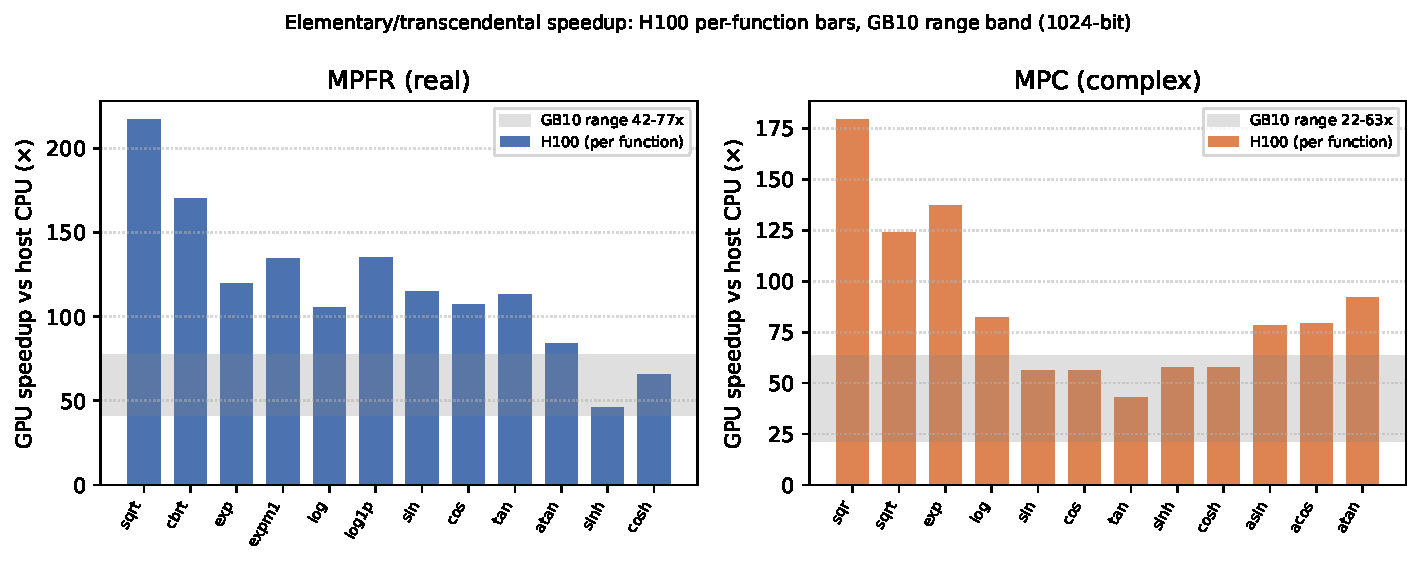
\includegraphics[width=0.95\textwidth]{figures/fig_h100_elem.pdf}
\caption{Elementary/transcendental GPU speedup over the host CPU. Bars = H100
per-function measurement; grey band = GB10 range (MPFR 42--77$\times$, MPC
22--63$\times$). Left: MPFR real; right: MPC complex. 1024-bit, all bit-exact.}
\label{fig:elemh100}
\end{figure}

\subsection{The fixed-precision fast path and a precision sweep}
\label{sec:sweep}

The fixed-precision path is far faster than the runtime path. For 1024-bit AXPY
(N=$2^{20}$), \code{cu\_freal} ran \textbf{142$\times$} faster than the existing
cu\_mpfr-GPU path and \textbf{352$\times$} faster than system CPU MPFR (both
bit-exact).

To expose the precision dependence, AXPY was swept with \code{make bench3}. GB10
was measured over 128--8192 bits (Table~\ref{tab:bench3}); the H100 sweep was
\textbf{extended to 128--65536 bits} so the fixed, runtime and CPU paths fully
cross (Table~\ref{tab:bench3h100}). The GB10 and H100 curves are overlaid in
Figure~\ref{fig:real} (real), Figure~\ref{fig:complex} (complex) and
Figure~\ref{fig:speedup} (speedup); solid = H100, dashed = GB10.

On GB10 the \code{cu\_freal} time is flat through 1024 bits (fully
register-resident), \textbf{jumps $\sim$7$\times$ at 2048 bits} (where the
$N=32$-limb significand spills from registers to local memory), and reaches parity
with one CPU core at 8192 bits. The complex side has the same shape with an even
larger lead (peak $\sim$48$\times$ vs cu\_mpc and $\sim$107$\times$ vs CPU at 1024
bits).

\begin{table}[h]
\centering
\caption{Precision sweep of the fixed-precision path (AXPY, N=4096, GB10, all bit-exact)}
\label{tab:bench3}
\begin{tabular}{rrrrrr}
\toprule
Bits & \code{cu\_freal} & \code{cu\_mpfr} & CPU & freal/cu\_mpfr & freal/CPU \\
\midrule
128  & 0.005 & 0.050 & 0.190 & 10.2$\times$ & 38.5$\times$ \\
256  & 0.005 & 0.088 & 0.222 & 19.6$\times$ & 49.1$\times$ \\
512  & 0.006 & 0.174 & 0.320 & 29.5$\times$ & 54.1$\times$ \\
1024 & 0.008 & 0.388 & 0.677 & 47.4$\times$ & \textbf{82.6$\times$} \\
2048 & 0.056 & 0.506 & 0.322 & 9.0$\times$  & 5.7$\times$ \\
4096 & 0.184 & 0.996 & 0.473 & 5.4$\times$  & 2.6$\times$ \\
8192 & 0.823 & 1.989 & 0.814 & 2.4$\times$  & \textbf{1.0$\times$} \\
\bottomrule
\end{tabular}\\[2pt]
\footnotesize Times in ms (8-iteration average).
\end{table}

\begin{figure}[h]
\centering
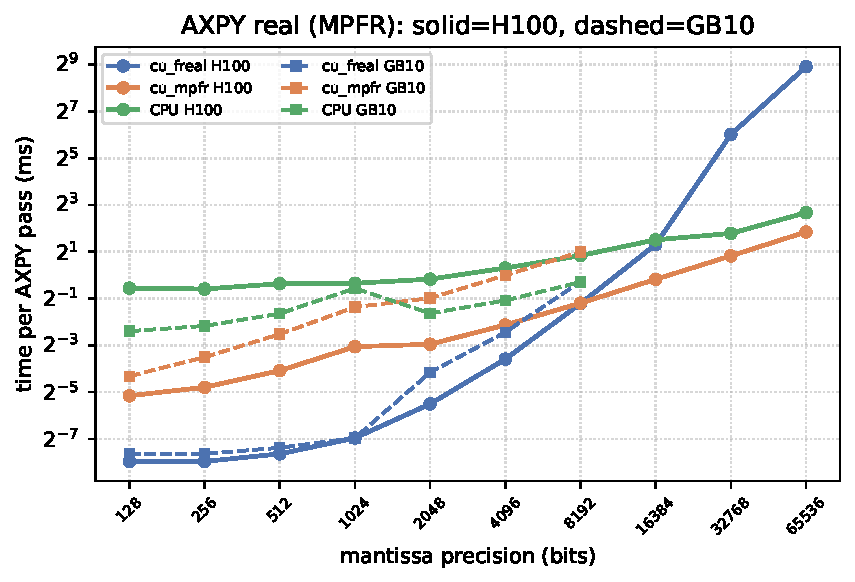
\includegraphics[width=0.95\textwidth]{figures/fig_bench3_real.pdf}
\caption{Real AXPY time vs precision (log-log). Solid = H100 (to 65536 bits),
dashed = GB10 (to 8192 bits); blue = \code{cu\_freal}, orange = \code{cu\_mpfr},
green = CPU. Fixed precision is flat through 1024 bits, jumps at 2048 (spill), and
on the H100 crosses \code{cu\_mpfr} at 8192 bits and the CPU at 16384 bits, then
diverges sharply.}
\label{fig:real}
\end{figure}

\begin{figure}[h]
\centering
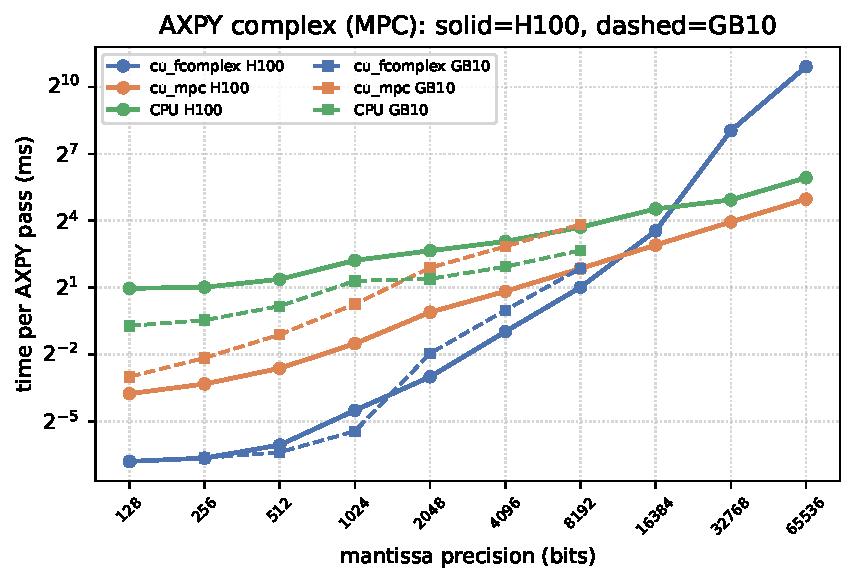
\includegraphics[width=0.95\textwidth]{figures/fig_bench3_complex.pdf}
\caption{Complex AXPY time vs precision (log-log); series as in
Figure~\ref{fig:real}. Same shape with a larger fixed-precision lead, but on the
H100 \code{cu\_fcomplex} crosses \code{cu\_mpc} at 16384 bits and the CPU before
32768 bits.}
\label{fig:complex}
\end{figure}

\begin{figure}[h]
\centering
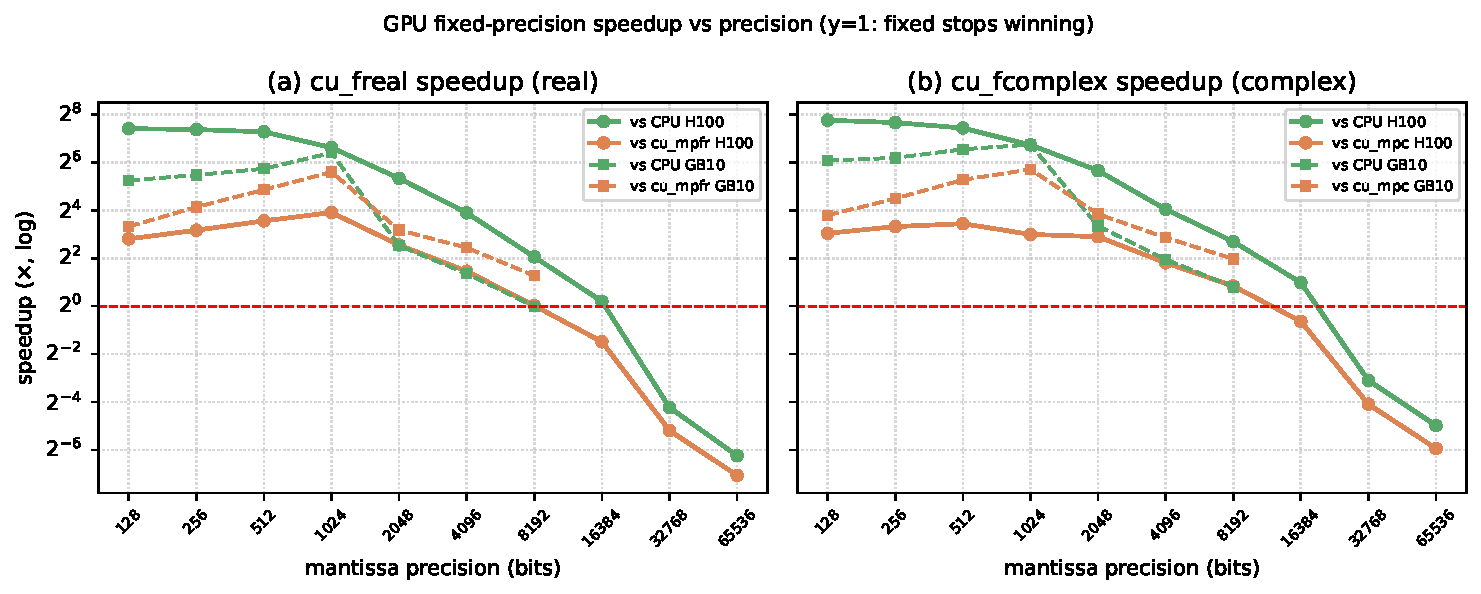
\includegraphics[width=0.98\textwidth]{figures/fig_speedup_gpu.pdf}
\caption{GPU fixed-precision speedup vs precision (log-log, $y=1$ is parity).
Solid = H100, dashed = GB10. (a) real (vs CPU and vs cu\_mpfr); (b) complex (vs CPU
and vs cu\_mpc). Peak at 1024 bits, spill knee at 2048 bits, and $y<1$ at high
precision where fixed precision loses.}
\label{fig:speedup}
\end{figure}

On the H100 the larger machine hides latency better, so two effects appear that
are consistent with the occupancy story of Section~\ref{sec:platform}
(Table~\ref{tab:bench3h100}). First, the \textbf{GPU runtime path}
(\code{cu\_mpfr}/\code{cu\_mpc}) is \textbf{$\sim$2--5$\times$ faster on the H100
than GB10 at every precision} (e.g.\ 1024-bit real: 0.120\,ms vs GB10's
0.388\,ms). Second, the H100's \textbf{fixed-precision spill knee at 2048 bits is
far softer}---\code{cu\_freal} rises only $\sim$2.75$\times$ from 1024 to 2048
bits (0.008$\to$0.022\,ms) versus GB10's $\sim$7$\times$ jump
(0.008$\to$0.056\,ms)---because the H100's larger register file and local-memory
bandwidth cushion the register$\to$local spill.

\paragraph{All paths cross (H100).}
Pushing the precision further, the fixed-precision advantage disappears entirely.
For real AXPY, \code{cu\_freal} reaches \textbf{parity with cu\_mpfr at 8192 bits}
(0.430 vs 0.436\,ms) and \textbf{crosses the CPU at 16384 bits} (2.477 vs
2.847\,ms), then degrades catastrophically (64.6\,ms at 32768, 482\,ms at 65536)
as the spilled schoolbook $O(n^2)$ thrashes local memory. The complex side has the
same shape: \code{cu\_fcomplex} crosses cu\_mpc at 16384 bits and the CPU before
32768 bits. Meanwhile the \textbf{GPU runtime path stays faster than the CPU even
at 65536 bits} (real 3.6 vs 6.4\,ms, complex 31.4 vs 60.9\,ms), showing that at
high precision the runtime path (or the sub-quadratic CPU) is preferable to the
fixed path. Every sweep point is bit-identical to the host (\code{rel}=0).

\begin{table}[h]
\centering
\caption{Precision sweep on the H100 (AXPY, N=4096, all bit-exact). GB10 is not
re-measurable here, so see Table~\ref{tab:bench3} for GB10 to 8192 bits. Times in
ms (8-iteration average).}
\label{tab:bench3h100}
\footnotesize
\begin{tabular}{rrrr@{\hskip 1.5em}rrr}
\toprule
 & \multicolumn{3}{c}{real (MPFR)} & \multicolumn{3}{c}{complex (MPC)}\\
\cmidrule(r){2-4}\cmidrule(l){5-7}
Bits & \code{cu\_freal} & \code{cu\_mpfr} & CPU & \code{cu\_fcplx} & \code{cu\_mpc} & CPU \\
\midrule
128   & 0.004   & 0.028 & 0.681 & 0.009    & 0.074  & 1.955 \\
256   & 0.004   & 0.036 & 0.663 & 0.010    & 0.100  & 2.029 \\
512   & 0.005   & 0.059 & 0.776 & 0.015    & 0.163  & 2.595 \\
1024  & 0.008   & 0.120 & 0.786 & 0.044    & 0.351  & 4.670 \\
2048  & 0.022   & 0.129 & 0.888 & 0.125    & 0.932  & 6.309 \\
4096  & 0.083   & 0.228 & 1.235 & 0.509    & 1.785  & 8.403 \\
8192  & 0.430   & 0.436 & 1.787 & 2.025    & 3.626  & 13.105 \\
16384 & 2.477   & 0.884 & 2.847 & 11.693   & 7.529  & 23.115 \\
32768 & 64.635  & 1.769 & 3.443 & 263.499  & 15.429 & 30.636 \\
65536 & 482.420 & 3.601 & 6.375 & 1929.433 & 31.360 & 60.912 \\
\bottomrule
\end{tabular}\\[2pt]
\footnotesize Crossover points: real \code{cu\_freal}$\approx$\code{cu\_mpfr} at
8192 bits and \code{cu\_freal}$>$CPU at 16384 bits; complex
\code{cu\_fcplx}$\approx$\code{cu\_mpc} at 16384 bits.
\end{table}

\subsection{The fixed-precision path on the CPU}

\code{cu\_freal}/\code{cu\_fcomplex} are header-only and compile/run on the host
with g++ alone (using \code{\_\_int128}). On the CPU (single thread) versus system
MPFR/MPC, they are \textbf{faster only at low precision} (Table~\ref{tab:cpu}).
\code{cu\_freal}'s multiply is schoolbook $O(n^2)$, whereas GMP/MPFR is
sub-quadratic (Karatsuba/Toom/FFT); the GPU won because register-residency and
massive parallelism hid the $O(n^2)$ cost, an advantage a single CPU thread lacks,
so above $\sim$512 bits the algorithmic gap shows.

\begin{table}[h]
\centering
\caption{CPU-only fixed precision vs system MPFR/MPC (AXPY, N=4096, single thread; ratio $>1$ means fixed precision is faster)}
\label{tab:cpu}
\begin{tabular}{rrr}
\toprule
Bits & freal/MPFR & fcplx/MPC \\
\midrule
128  & \textbf{1.28$\times$} & \textbf{1.79$\times$} \\
256  & \textbf{1.23$\times$} & \textbf{1.48$\times$} \\
512  & 1.03$\times$ & 0.99$\times$ \\
1024 & 0.71$\times$ & 0.67$\times$ \\
2048 & 0.09$\times$ & 0.17$\times$ \\
4096 & 0.03$\times$ & 0.06$\times$ \\
8192 & 0.01$\times$ & 0.03$\times$ \\
\bottomrule
\end{tabular}
\end{table}

\begin{figure}[h]
\centering
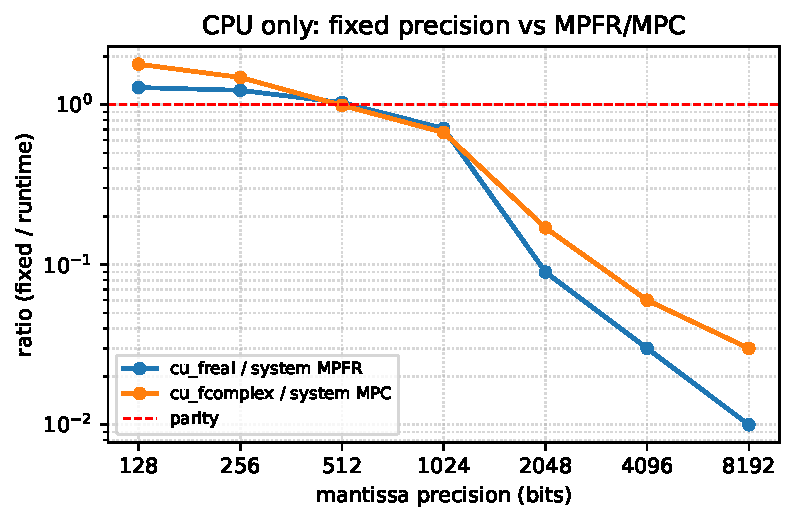
\includegraphics[width=0.82\textwidth]{figures/fig_cpu_crossover.pdf}
\caption{CPU-only fixed precision vs MPFR/MPC ratio (log $y$, $y=1$ is parity).
Fixed precision wins only at 128--256 bits; at high precision MPFR/MPC with its
sub-quadratic multiply wins.}
\label{fig:cpu}
\end{figure}

\subsection{Discussion}

On the GPU the register-resident fixed-precision path \textbf{wins decisively up to
$\sim$1024 bits} (up to $\sim$83$\times$ vs CPU, $\sim$142$\times$ vs cu\_mpfr-GPU),
hits a spill knee at 2048 bits, and reaches CPU parity at 8192 bits. On a single
CPU thread the same path beats MPFR/MPC only at 128--256 bits. Hence the
fixed-precision schoolbook advantage is bounded by \textbf{(i) GPU parallelism and
(ii) low/medium precision}; for high precision or on the CPU, MPFR/MPC with its
sub-quadratic multiply is preferable.

\subsection{Cross-platform comparison: GB10 vs H100 (synthesis)}
\label{sec:platform}

Finally we collect, from the two-GPU viewpoint, the results reported side by side
throughout this section. The six runtime-precision demos (real/complex AXPY,
matrix--vector and matrix multiply) were run on both machines from the same source
at the same problem sizes and 1024-bit precision, all bit-exact. Because the two
hosts use different CPUs (GB10's Grace ARM vs the H100 box's x86), the \textbf{GPU
time in ms} is the fair hardware-to-hardware metric; the GPU-vs-CPU speedups are
listed for completeness but each is relative to its own host
(Table~\ref{tab:platform}, Figure~\ref{fig:platform}).

\begin{table}[h]
\centering
\caption{GB10 vs H100, runtime-precision demos (1024 bits, all bit-exact). The
ratio is GB10/H100 GPU time ($>1 \Rightarrow$ H100 faster).}
\label{tab:platform}
\begin{tabular}{lrrrr}
\toprule
Demo & $N$ & GB10 GPU & H100 GPU & H100/GB10 \\
\midrule
AXPY MPFR    & 16384 & 1.17\,ms  & 0.295\,ms & \textbf{3.97$\times$} \\
AXPY MPC     & 16384 & 4.81\,ms  & 1.037\,ms & \textbf{4.64$\times$} \\
matvec MPFR  & 256   & 11.3\,ms  & 15.80\,ms & 0.72$\times$ \\
matvec MPC   & 128   & 24.4\,ms  & 29.68\,ms & 0.82$\times$ \\
matmul MPFR  & 96    & 23.0\,ms  & 12.00\,ms & \textbf{1.92$\times$} \\
matmul MPC   & 64    & 27.9\,ms  & 15.63\,ms & \textbf{1.79$\times$} \\
\bottomrule
\end{tabular}
\end{table}

\begin{figure}[h]
\centering
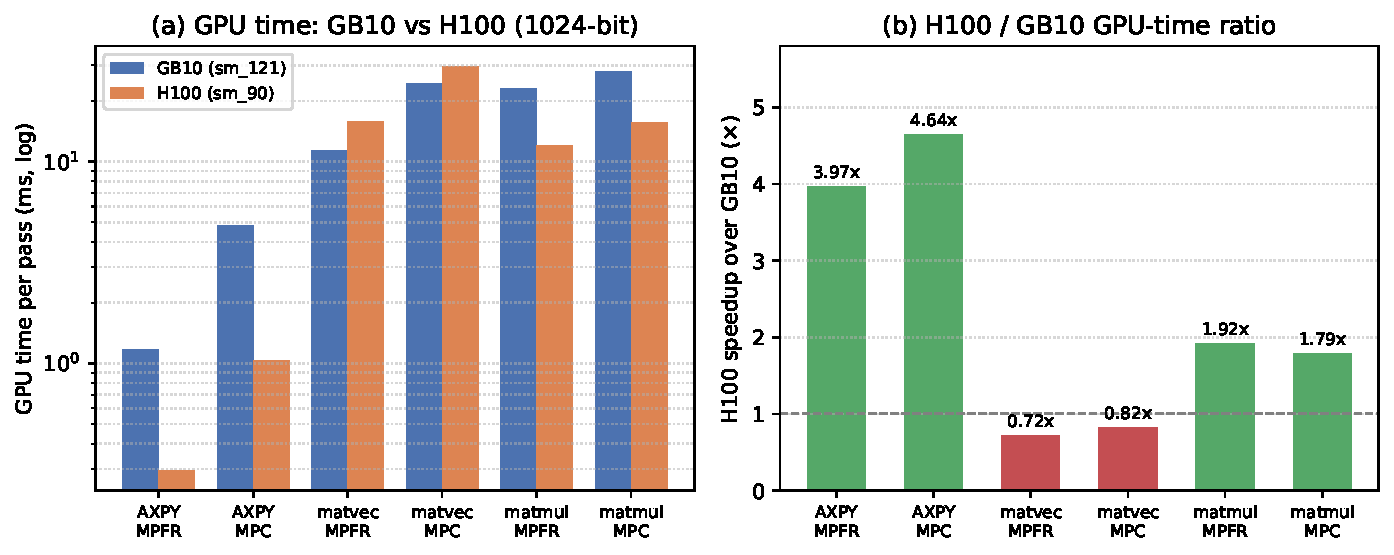
\includegraphics[width=0.98\textwidth]{figures/fig_gb10_vs_h100.pdf}
\caption{GB10 vs H100. (a) GPU time per pass (log scale); (b) H100 speedup over
GB10 ($y=1$ is parity). The H100 wins the high-parallelism kernels but loses the
small-$N$ matvec.}
\label{fig:platform}
\end{figure}

The pattern is consistent and explainable by occupancy. The H100 dominates the
\textbf{high-parallelism} kernels---AXPY ($\sim$4$\times$, memory-bandwidth bound
over 16384 elements) and matrix multiply ($\sim$1.8--1.9$\times$, an $O(N^2)$ grid
that saturates the device)---where its 132 SMs and HBM3 bandwidth are fully used.
It \textbf{loses} the matrix--vector kernels (0.72--0.82$\times$): with one thread
per output row and $N=128$--256, only $\sim$128--256 threads are ever active, so
the launch is \textbf{occupancy-starved} and the result is bound by the
single-thread latency of one long multiple-precision dot product, where the newer
GB10 core (\code{sm\_121}, higher clock) is faster. Figure~\ref{fig:platspeedup}
shows the GPU-vs-CPU speedups on the two platforms side by side.

\begin{figure}[h]
\centering
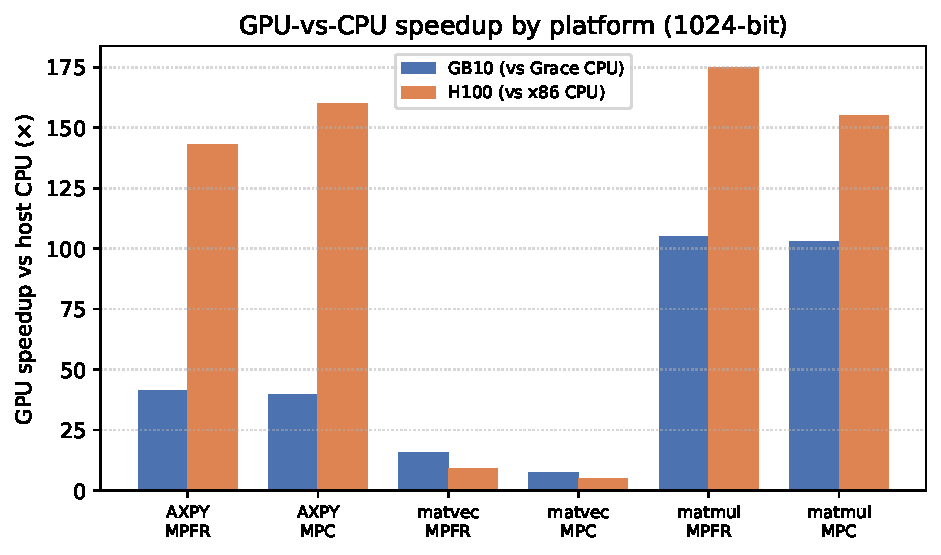
\includegraphics[width=0.7\textwidth]{figures/fig_platform_speedup.pdf}
\caption{GPU-vs-CPU speedup by platform (each GPU against its own host CPU),
1024-bit. The H100's higher AXPY/matmul speedups partly reflect its faster GPU
and partly its different (x86) host baseline.}
\label{fig:platspeedup}
\end{figure}

The \textbf{elementary functions} (Table~\ref{tab:elemh100},
Figure~\ref{fig:elemh100}) show the same picture: the $N=4096$ evaluation fills the
device, so both machines are fast---the H100 reaches \textbf{43--217$\times$} per
function (vs its x86 host) and the GB10 spans \textbf{42--77$\times$} (MPFR) /
\textbf{22--63$\times$} (MPC, vs the Grace ARM). The speedups are each relative to
their own host and so not directly comparable, but both machines peak on the cheap
kernels (\code{sqrt}, \code{cbrt}, \code{sqr}) and bottom out on the heavy multi-AGM
kernels (\code{log}, complex \code{asin}/\code{acos}).

The \textbf{precision sweep} (Section~\ref{sec:sweep}) is consistent with the same
occupancy effect: at $N=4096$ the H100 hides latency better, so its runtime path is
$\sim$2--5$\times$ faster at every precision and its fixed-precision spill knee at
2048 bits is softer ($\sim$2.75$\times$ vs GB10's $\sim$7$\times$).

In short, the H100 is the better device when there is enough parallelism to fill it
(high-parallelism AXPY, matrix multiply, elementary functions, large-$N$ sweep),
while the GB10 is competitive in the latency-bound small-$N$ regime (matrix-vector).

%======================================================================
\section{Conclusion and Future Work}
\label{sec:conclusion}

GMP(mini-gmp)/MPFR/MPC were \textbf{faithfully} ported into CUDA kernels via
re-runnable transform scripts, and real (MPFR) and complex (MPC) AXPY were
accelerated by $\sim$40$\times$ while remaining bit-identical to the CPU. The crux
of the port was making it compile (NORETURN/NO\_ASM/realloc/\_Complex), making it
run on the device (RODATA/managed globals/allocation routing/constant caches),
and substituting an \code{mpz}-based \code{mpfr\_div} for the device miscompile.
Stack limits, the bump arena, parallelism, and coexistence (the cu\_ namespace and
umbrella) were also addressed.

In addition, a compile-time fixed-precision, register-resident
\code{cu\_freal<PB>}/\code{cu\_fcomplex<PB>} and fixed-precision elementary
functions were introduced. These beat MPFR/MPC by orders of magnitude at
low/medium precision on the GPU, and the precision sweep quantified the crossover:
\textbf{2048 bits is the spill knee, and CPU parity is reached at 8192 bits}.
A cross-platform comparison (GB10 vs H100 NVL) further showed that the runtime-precision
kernels are \textbf{occupancy-bound}: the H100 is $\sim$4$\times$ (AXPY) and
$\sim$1.8--1.9$\times$ (matmul) faster where there is enough parallelism to fill its
132 SMs, but the small-$N$ matrix--vector kernels stay latency-bound and slightly
favour the GB10.

Future work includes fixed-precision implementations of the MPFR/MPC special
functions (gamma, zeta, erf, Bessel, \dots), reducing register pressure and
compile time at high precision, adding sub-quadratic multiplication (Karatsuba,
etc.) to the fixed-precision path, and fully race-free per-thread exponent/flag
state.

\bigskip
\noindent\textbf{Reproduction}: \code{./configure \&\& make}; \code{make check}
(minigmp/mpfr/mpc/trans bit-exactness), \code{make demos}/\code{matrix}/\code{bench}
(performance), \code{make sample-fixed}/\code{check-fixed}/\code{check-fmath}/\code{bench3}
(fixed precision). The CPU-reference targets (\code{bench3}, \code{coexist},
\code{cputest}, \code{cpubench}) need a system GMP/MPFR/MPC; if it lives in a
non-standard prefix, pass \code{./configure --with-mp-prefix=DIR} (e.g.\
\code{\textasciitilde/local}), which adds its \code{include}/\code{lib} (with
rpath) to the build. The target GPU is selected with
\code{--with-cuda-arch=ARCH} (default \code{sm\_90}; the GB10 runs used
\code{sm\_121}). See the user manuals \code{doc/manual.md} (English) /
\code{doc/manual.ja.md} (Japanese) for details.

\end{document}
